\documentclass[30pt,twocolumn,letterpaper]{article}
\usepackage{cvpr}
\usepackage{times}
\usepackage{booktabs}
\usepackage{epsfig}
\usepackage{graphicx}
\usepackage{amsmath}
\usepackage{amssymb}
\cvprfinalcopy
\def\cvprPaperID{****}
\def\httilde{\mbox{\tt\raisebox{-.5ex}{\symbol{126}}}}
\usepackage{graphicx}
\usepackage{indentfirst}
\setlength{\parindent}{2em}
\usepackage{cite}
\usepackage[colorlinks,linkcolor=red,anchorcolor=blue,citecolor=green,backref=page]{hyperref}
\author{Qilei Zhang\\\\
Jun 24 2018}
\title{Semantic Style Transfer and Turning Two-Bit Doodles into Fine Artwork}
\begin{document}
\maketitle
\begin{abstract}
  Convolutional neural networks have proven highly effective at image synthesis and style transfer. For most users, it may be a challenging task to use them as a tool, because their unpredictable behavior is contrary to ordinary intuition.
\end{abstract}
\section{Introduction}
Because of the training of CNNs for image classification, we extract basic patterns from large data sets. Compared with the original pixel level, the deep layer of the network provides more expressive feature space, which is useful not only for classification, but also for generation\cite{Beebee2010Transfer}. \\
\begin{figure}[htbp]
\small
\centering
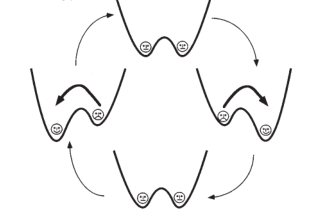
\includegraphics[width=20em]{000.png}
\caption{Synthesizing paintings with deep neural networks
via analogy. (a) Original painting by Renoir, (b) semantic
annotations, (c) desired layout, (d) generated output.}
\label{fig:lable}
\end{figure}\\
\section{Related Work}
The image analogy algorithm is able to transfer artistic style using pixel features and their local neighborhoods\cite{Diester2010Numerical}. The nearest algorithm using a deep neural network produces better quality results from the stylistic perspective, but this technique allows users to synthesize new images based on simple annotations\cite{Robert2012Focus}.\\
\begin{figure}[htbp]
\small
\centering
\includegraphics[width=20em]{001.png}
\caption{Deep image analogy for a Monet painting based on a doodle; it��s effectively semantic style transfer with no content loss. This result was achieved in only eight attempts, showcasing the potential for the algorithm as an interactive tool.}
\label{fig:lable}
\end{figure}\\
\section{Conclusion}
The existing style transfer technology is well performed. When the color and accuracy are not much related to the output image, or when the two image patterns are already similar, the attractiveness and applicability of the algorithm are reduced\cite{Thomas1969Paired}The example shown in the style transfer in this article shows how this technique helps to deal with completely opposite patterns in the corresponding image area, and analyzes how it helps users better control the output of these algorithms.
{\small
\bibliographystyle{ieee}
\bibliography{1}
}
\end{document}
